%Dokumenteigenschaften
\documentclass[a4paper, hidelinks, 12pt]{article}
%import
\usepackage{blindtext}
\usepackage{hyperref}
\usepackage{pdfpages}
\usepackage{amsmath}
\usepackage{amssymb}
\usepackage[b]{esvect}
\usepackage{listings}
\usepackage{xcolor}
\usepackage{pythontex}
\hypersetup{linktoc=all}
\lstset{language=Python}
\definecolor{code}{rgb}{255,255,255}
\definecolor{background}{rgb}{0,0,0}
\lstdefinestyle{mystyle}{backgroundcolor=\color{background}, }
\lstset{basicstyle = \small, breaklines=true, numbers=left}
\begin{document}
%Titelseite
\begin{titlepage}
\title{\Large{\textbf{\underline{Simulation von Boids}}}\linebreak\large\textbf{nach Craig Reynolds}}
\author{Oliver Fritzler}
\date{\today}
\maketitle
\end{titlepage}

%Inhaltsverzeichnis
\title{\Large{\textbf{\underline{Inhaltsverzeichnis}}}}
\tableofcontents
%UML-Diagramm
\section{UML-Diagramm}
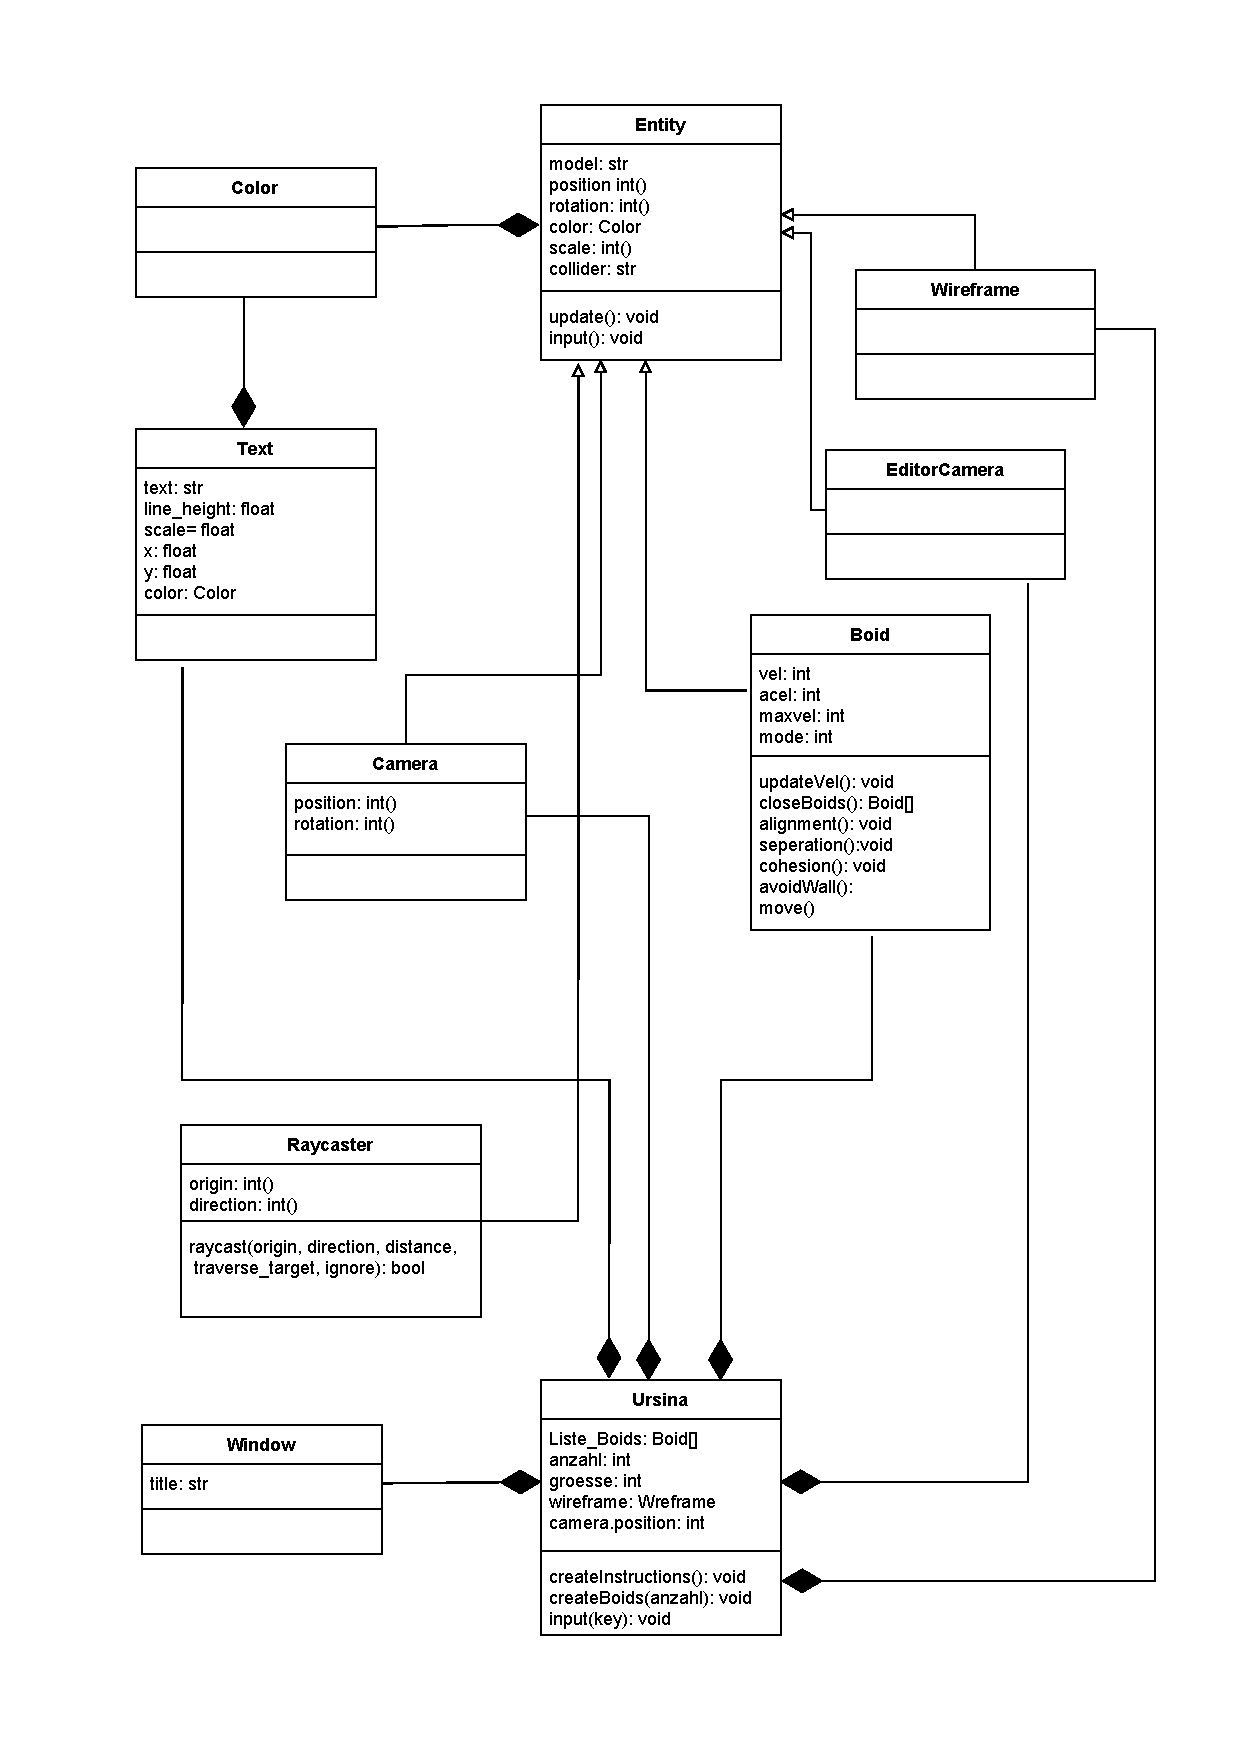
\includegraphics[scale=0.75, page=1]{UML/Boids_UML.pdf}
\newpage
%Grundidee
\section{Grundidee}
\subsection{Umgebung}
Die Programmiersprache \emph{\textbf{Python}} war vorgegeben, die Bibliothek zur grafischen Darstellung war frei überlassen. Aufgrund der einfachen und verständlichen Syntax, fiel die Auswahl auf die \emph{\textbf{ursina engine}}, welche auf der \emph{\textbf{panda3D engine}} basiert. Ursina ermöglicht es neben vorgegebenen Modellen auch blender-Dateien als Modelle für die einzelnen Objekte zu verwenden. Diese Objekte werden dargestellt und durch spezifische Funktionen (\textbf{update()}, \textbf{move()}, \textbf{input()}) jedes Bild aktualisiert. Dadurch kann man sowohl die Position durch Addition verändern, als auch Eingaben des Benutzers verarbeiten. 
	
\subsection{Darstellung des Raumes}
Zur Darstellung des Raumes werden 12 Objekte in Form eines Würfels erstellt, jedoch werden diese dann so skaliert, dass sie die Form eines Rechteckes annehmen. Diese werden dann so angeordnet, dass sie die Kanten eines Würfels bilden. 
Des Weiteren werden die Seitenflächen erstellt. Dabei werden wie davor 6 Objekte in Form eines Würfels erstellt. Nur werden diese jetzt so skaliert, dass sie eine quadratische Fläche bilden. Um diese unsichtbar zu machen wird der Sichtbarkeitswert auf Null gesetzt.
		
\subsection{Allgemeines zu den Boids}
Boids sind Körper, die sich Bewegen. Zur Veranschaulichung der Richtung sollten die Boids einen Körper mit einer Spitze haben, wie zum Beispiel ein Kegel. Da ein Kegel sehr viele Seiten hat, die alle jedes Bild berechnet werden müssen und dadurch die Performance senken, sollte man auf einen einfacheren Körper mit Spitze zurückgreifen, wie eine Pyramide. Diese Körper bewegen sind jedoch nicht chaotisch, da sie sich an \hyperref[sec:Regel]{\textbf{\emph{drei Regeln}}} handeln, die später erklärt werden.\linebreak
\newpage
\textbf{\underline{Verhalten an Wänden}}\label{sec:Verhalten}
Das Verhalten der Boids an den Wänden kann man auf verschiedene Weise gestalten. In dieser Simulation wurden drei davon versucht umzusetzen. 
\begin{enumerate}
\item \underline{\textbf{Warp}}\linebreak\label{sec:Warp}
Bei dieser Umsetzung werden die Boids bei Kontakt mit einer Wand auf die gegenüberliegende Seite "teleportiert".
			
\item \underline{\textbf{Wände vermeiden}}\linebreak\label{sec:AvoidWall}
Dabei drehen die Boids vor Kontakt mit einer Wand ab.
			
\item \underline{\textbf{PONG}}\linebreak\label{sec:Pong}
Hier verhalten sich die Boids, wie der Ball im Spiel \textbf{"PONG"}, d.h. sie bewegen sich auf die Wand in einem bestimmten Winkel zu und verlassen diese Wand dann in dem gleichen Winkel, nach dem \emph{Einfallswinkel-gleich-Ausfallswinkel-Prinzip}
\end{enumerate}

\subsection{Regeln}\label{sec:Regel}
Boids sind Objekte die sich in einem Raum bewegen. Dabei verfolgen sie drei Grundregeln:
\begin{itemize}
\item\textbf{\underline{Seperation}}\linebreak\label{sec:Seperation}
Diese Regel besagt, dass jeder einzelne Boid versucht, keinen anderen Boid zu treffen. 
\item\textbf{\underline{Alignment}}\linebreak\label{sec:Alignment}
Diese Regel besagt, dass jeder Boid versucht, in die selbe Richtung wie ein anderer sich zu bewegen. Dadurch entsteht ein sogenannter \textbf{"Flock"} also ein Schwarm von Boids.
\item\textbf{\underline{Coheseion}}\linebreak\label{sec:Cohesion}
Diese Regel besagt, dass die Boids in die Mitte des Schwarms steuern.
\end{itemize}
	
\subsection{Eingabe}
Der Benutzer soll durch Bewegen der Maus die Kamera rotieren können und durch Tastendruck die Kamera bewegen können. Außerdem soll es ihm ermöglicht werden die Anzahl der Boids und deren Verhalten zu ändern.
\newpage
	
	
	
\section{Umsetzung}
\subsection{Allgemein}
Aufrgund der Umsetzung der Eigesnchaften ist es nicht möglich die Darstellungsebene und die Informationsebene in verschiedene Dateien aufzuteilen. Es würde ein Import-Fehler auftreten, da die Liste aus der Darstellungsebene in die Informationsebene importiert werden müsste und die Klasse aus der Informationsebene in die Darstellungsebene.
	
\subsection{Fenster}\label{sec:Fenster}
Mit dem Aufrufen der Klasse \textbf{\emph{Ursina}} wird ein Fenster erschaffen, welches am Ende ausgeführt wird, mit all den benötigen Grafiken. Diesem Fenster kann man einen Titel vergeben, welche dann als Task angezeigt wird. Diese Klasse hat wie jede andere Klasse in Ursina die Funktion \textbf{\emph{input()}}, mit deren Hilfe man die Eingabe des Benutzers verarbeiten kann, die in dieser Umsetzung \hyperref[sec:input]{\textbf{\emph{hier}}} nachzulesen sind. Um dem Benutzer die Nutzung der Simulation zu vereinfachen, erstellt man in der Funktion \textbf{\emph{createInstruction()}}, mit der Klasse \textbf{\emph{Text}} eine Beschreibung und skaliert und positioniert sie so, dass sie nicht im Vordergrund liegt.[Code]
\subsection{Raum}\label{Wireframe}
Die Klasse \textbf{\emph{Wireframe}} wird erstellt, welche von der \textbf{\emph{Entity}}-Klasse erbt. Diese Klasse beinhaltet insgesamt 18 andere Entitys. 12 davon sind Würfel die so skaliert und positioniert werden, dass sie die Kanten eines großen Würfels bilden. Die anderen 6 sind ebenfalls Würfel, welche jedoch so skaliert werden, dass sie quadratischen Flächen formen. Diese Flächen werden dann so positioniert, dass die Seitenflächen des großen Würfels bilden. Da diese Seitenflächen nicht nötig zu sehen sind, kann man entweder den $\alpha$-Wert der Farbe oder den $\alpha$-Wert einzeln auf 0 setzen, beide Werte sind die Sichtbarkeitswerte. Bei dieser Umsetzung wird letzteres angewandt. Sowohl den Kanten, als auch den Seitenflächen wird eine Box als Kollisionskörper unter \emph{collider} zugeteilt, damit die Boids daran abprallen können[Code] \newline Warum diese Klasse erstellt werden muss, wird im Teil \hyperref[sec:seperation]{\textbf{\emph{seperation()}}} erklärt. 
\subsection{Boids}\label{sec:Boid}
Die Darstellung der Boids erfolgt durch die Implementierung der gleichnamigen Klasse \textbf{\emph{Boid}}. Diese Klasse erbt von der Klasse \textbf{\emph{Entity}}, welche laut den Entwicklern von Ursina die \emph{"god class"} ist. 
Den Boids wird eine selbsterstellte .blender-Datei als Model gegeben. Dieses Model gleicht einer Pyramide. Die Farbe dieser Pyramide wird mithilfe des \emph{random\textunderscore color()} Befehls der Klasse \textbf{\emph{color}} festgelegt, welche innerhalb \emph{self.color} gespeichert wird. Des Weiteren speichert der Boid seine Position sowohl in einem Tuple unter \emph{self.position} und als auch in drei einzelnen Variablen \emph{self.x}, \emph{self.y} und \emph{self.z}. Um die Bewegung zu ermöglichen wird dem Boid eine Ausrichtung gegeben, die er unter \emph{self.rotation} speichert. Um die Geschwindigkeit zu variieren wird die Geschwindigkeit, die Beschleunigung und die zu maximal erreichende Geschwindigkeit unter \emph{self.vel}, \emph{self.acel} und \emph{self.maxVel} gespeichert. Um das Verhalten an den Wänden zu ändern, speichert der Boid den aktuellen Modus unter \emph{self.mode}. Damit der Boid die \textbf{Raycasts} der anderen Boids auslösen kann, wird dem Boid ein Körper zugeteilt der dies ermöglicht, welcher unter \emph{self.collider} gespeichert wurde. Den Boids wird eine Box zugeteilt, da die von den vorgegebenen Beispielen am passendsten sind.
Nach dem Konstruktor werden die Getter, die die Werte der Eigenschaften zurückgeben und die Setter, die die Werte der Eigenschaften überschreiben, deklariert.
Im folgenden werden die weiteren Funktionen erklärt:\newline
	
\underline{\textbf{updateVel()}}\label{sec:updateVel}
Damit sich die Boids nicht mit der selben Geschwindigkeit bewegen, wird hier die Geschwindigkeit mithilfe der Addition der Beschleunigung \emph{self.acel} erhöht.
\newline
		
\underline{\textbf{closeBoids()}}\label{sec:closeBoids}
Damit der Boid sich an die vorgegebenen Regeln halten kann, muss er wissen welche Boids sich in seiner Nähe befinden. Dafür wird in dieser Funktion die Liste in der alle Boids gespeichert wurden (siehe \hyperref[sec:createBoids]{\emph{\textbf{createBoids()}}}) durchgegangen und überprüft ob die Distanz in zwischen dem Boid und dem zu vergleichenden Boid unter einem bestimmten Wert liegt. Falls dies zu trifft wird der zu vergleichende Boid in eine Liste hinzugefügt, die alle Boids in der Nähe beinhaltet. Diese Liste wird am Ende zurückgegeben. Mithilfe dieser Funktion wird dem Boid ein gewisser Sichtbereich gegeben, da er nicht weiter als der festgelegt Wert "sehen" kann.[Code]
\newline
		
\underline{\textbf{alignment()}}\label{sec:alignment}
Diese Funktion ist dazu da um die \hyperref[sec:Alignment]{2. Regel \textbf{\emph{"Alignment"}}} zu befolgen. Dafür werden anfangs die Boids in der Nähe mithilfe der \hyperref[sec:closeBoids]{\emph{\textbf{closeBoids()}}}-Funktion bestimmt, und in der \emph{proximity}-Liste gespeichert. Darauf werden alle Werte die etwas mit der Bewegung zu tun haben, d.h. sowohl die Rotationswerte als auch alle Werte der Geschwindigkeit des Boids gespeichert. Das Selbe wird nun mit jedem Boid gemacht der in der \emph{proximity}-Liste gespeichert ist. Für jeden gespeicherten Wert wird der Durchschnitt berechnet. Nach der Berechnung werden die Eigenschaften mit diesen Durchschnittswerten überschrieben.
\newline\newline
		
\underline{\textbf{seperation()}}\label{sec:seperation}
Mithilfe dieser Funktion versucht der Boid die \hyperref[sec:Seperation]{1. Regel \textbf{\emph{"Seperation"}}} zu befolgen. 
Bei dieser Funktion gibt es 2 Umsetzungsversuche:\newline 
\begin{itemize}
	\item \textbf{Versuch 1}\newline Wiedermal werden die Boids in der Nähe in der \emph{proximity}-Liste durch die \hyperref[sec:closeBoids]{\textbf{\emph{closeBoids()}}}-Funtktion gespeichert. Nun wird die Distanz zwischen dem Boid und dem zu vergleichenden Boid überprüft und falls diese in einem kleinen Bereich liegt, wird die Differenz des Abstands und der eigenen Position multipliziert mit 0.5, der eigenen Position hinzuaddiert damit die beiden Boids an Abstand gewinnen.
	\item \textbf{Versuch 2}\newline
	Bei diesem Versuch werden 5 \textbf{\emph{Raycasts}} erstellt, die nach vorne, hinten, oben, rechts und links gerichtet sind. Diese haben eine sehr kurze Distanz und ignorieren die \hyperref[Wireframe]{\textbf{\emph{Wireframe}}}-Klasse, da sie nur von Boids ausgelöst werden können. Falls einer dieser \textbf{\emph{Raycasts}} ausgelöst wird, wird die Rotation in die entgegengesetzte Richtung durch Addieren des Produkts aus Richtung und Geschwindigkeit. Diese Umsetzung ist der Grund für die Erstellung der \hyperref[Wireframe]{\textbf{\emph{Wireframe}}}-Klasse
\end{itemize}  

\textbf{Anmerkung:}
Der Versuch 1 scheint nicht zu funktionieren, da es oft vorkommt, dass Boids ineinander liegen. Um die zu umgehen, habe ich sowohl versucht den Vorfaktor zu ändern, was im chaotischen Rotieren resultierte, als auch durch Veränderung der Differenz, welches nichts änderte
Der Versuch 2 ist aufgrund der Raycasts sehr ressourcenfressend, weswegen ich empfehle den Versuch 2 auszukommentieren und den Versuch 1 zu entkommentieren.
Des Weiteren kann das nicht Funktionieren an der \hyperref[sec:cohesion]{\textbf{\emph{cohesion()}}}-Funktion liegen, die als Gegenspieler agiert.
\newline\newline

\underline{\textbf{cohesion()}}\label{sec:cohesion}
Diese Funktion dient dazu, dass der Boid die \hyperref[sec:Cohesion]{3. Regel \textbf{\emph{"Cohesion"}}} befolgt. Sie funktioniert ähnlich wie \hyperref[sec:seperation]{\textbf{\emph{seperation()}}}, nur leicht abgewandelt. Anstatt die Distanz mit jedem Boid abzugleichen, wird hier zuerst ein Mittelpunkt aller Boids eines \emph{Flocks} berechnet. Falls die Distanz zwischen diesem Mittelpunkt und der Position des Boids über einem bestimmten Wert liegt, wird die Differenz des Mittelpunkts und der eigenen Position multipliziert mit 0.5, der eigenen Position abgezogen. Dadurch bewegt sich der Boid weiter in die Mitte des \textbf{Flocks}.
\newline\newline


		
\underline{\textbf{avoidWall()}}\label{sec:avoidWall}
Diese Funktion verändert das Verhalten der Boids in der Nähe der Wände. Dafür erstellt der Boid einen \textbf{Raycast}, der in Bewegungsrichtung gerichtet ist. Falls dieser \textbf{Raycast} etwas berührt werden vier weitere erstellt, nur dieses Mal nach nach vorne, hinten , rechts und links gerichtet. Danach wird nach dem Herausfinden der \emph{kleinsten} Differenz entschieden, in welche Richtung die Rotation durch Multiplikation verändert wird.
\textbf{Anmerkung:} Bei dem Versuch es zu implementieren, ist mir aufgefallen, dass die Boids durch die Wände schreiten und nie umdrehen. Die einzige logische Möglichkeit, womit ich dies erklären, kann ist das durch die \hyperref[sec:move]{\textbf{\emph{move()}}}-Funktion die Boids die Wände überspringen und dadurch der \textbf{Raycast} nicht aktiviert wird. Man könnte es versuchen zu lösen, indem man bei Überschreitung die Position überschreibt, damit die \textbf{Raycasts} eventuell auslösen.
\newline\newline
	
\underline{\textbf{move()}}\label{sec:move}
Diese Funktion ermöglicht die Fortbewegung des Boids durch Addition des Produkts aus der Bewegungsrichtung und der Geschwindigkeit dividiert durch 1000. Des Weiteren wird die Geschwindigkeit erhöht, durch den Aufruf der \hyperref[sec:updateVel]{\textbf{\emph{updateVel()}}}-Funktion.
In dieser Funktion wird neben der Bewegung auch das Verhalten an den Wänden bestimmt durch Abgleichung des Moduswertes.\newline
	\begin{itemize}
\item Falls dieser Wert auf 1 liegt, wird der \hyperref[sec:Warp]{\textbf{\emph{"Warp"}}} verwendet, welcher die aktuellen Positionswerte mit den Grenzwerten abgleicht. Falls die Positionswerte diese Grenzwerte überschreiten, wird die Position auf die gegenüberliegende Seite gelegt.
\item Falls der Moduswert auf 2 liegt, wird das \hyperref[sec:AvoidWall]{\textbf{\emph{"Wände vermeiden"}}-Verhalten} aufgerufen und die \hyperref[sec:avoidWall]{\textbf{\emph{avoidWall()}}}-Funktion aufgerufen.
\item Falls der Wert auf 3 liegt, wird der \hyperref[sec:Pong]{\textbf{\emph{"PONG"}}-Modus} aufgerufen. Dabei wird versucht bei Überschreitung der Grenzwerte bestimmte Rotationswerte nach dem "Einfallswinkel entspricht Ausgleichswinkel"-Prinzip zu ändern, dies hat jedoch mithilfe der Rechnung *-1-180 oder anderen Methoden nicht funktioniert, da es zu viele Spezialfälle gibt um es allgemein zu verfassen, und außerdem vermute ich, dass es ebenfalls aufgrund des Gimble-Locks ebenfalls nicht funktioniert.
\end{itemize}
		
\underline{\textbf{update()}}\label{sec:update}
Da diese Funktion jedes Bild automatisch aufgerufen wird, ruft sie alle nötigen Funtkonen auf. D.h. \hyperref[sec:move]{\textbf{\emph{move()}}}, \hyperref[sec:cohesion]{\textbf{\emph{cohesion()}}}, \hyperref[sec:seperation]{\textbf{\emph{seperation()}}} und \hyperref[sec:alignment]{\textbf{\emph{alignment()}}}.
		
	
\subsection{Funktionen im Fenster}
\textbf{createBoids()}\label{sec:createBoids}
Diese Funktion wird vom \hyperref[sec:Fenster]{\textbf{\emph{Fenster}}} aufgerufen und erstellt für die festgelegt Anzahl \hyperref[sec:Boid]{\textbf{\emph{Boids}}} mit einer festgelegten Größe und speichert diese in \emph{Liste\textunderscore Boids}. Dabei wird dem Boid immer der Modus \textbf{1} gegebenen. Bei dem Versuch es mit einer Variable zu lösen, die den aktuellen Modus beinhalten, kam kein brauchbares Ergebnis heraus
	
		
\subsection{Eingabe}
\textbf{input()}\label{sec:input}
Wie auch die \hyperref[sec:update]{\textbf{\emph{update()}}}-Funtkion wird die input()-Funktion jedes Bild automatisch aufgerufen. Diese gleicht ab welche Taste gedrückt wurde und führt Fälle aus.\newline Gedrückte Taste: 
\begin{enumerate}
\item \textbf{+/-} Beim Drück dieser Tasten, wird entweder ein \hyperref[sec:Boid]{\textbf{\emph{Boid}}} erstellt und der Liste angehängt oder der letzte Boid wird deaktiviert und aus der Liste gelöscht. Er muss deaktiviert werden, da er sonst immer noch dargestellt werden würde.
\item \textbf{1,2,3} Beim Druck einer dieser Tasten wird der das \hyperref[sec:Verhalten]{\textbf{\emph{Verhalten}}} jedes einzelnen Boids durch Änderung der Modus-Eigenschaft in einer for-Schleife geändert.
		
\end{enumerate}
%wichtigste Funktionen
\newpage
\section{wichtigste Funktionen}
\subsection{Fenster}
\begin{lstlisting}
#Fenster wird erstellt
app = Ursina()
#Fenstertitel wird festgelegt
window.title = "Boids Simulation"
#Fenster wird ausgefuehrt
app.run()
\end{lstlisting}
\subsection{Kamera}
\begin{lstlisting}
#Kameraposition wird veraendert um den Bereich von Anfang an zu sehen
camera.position = (0,10,-350)
#EditorCamera ermoeglicht die Veraenderung der Kamera
EditorCamera()
\end{lstlisting}
\subsection{Wireframe}
\begin{lstlisting}
#Erzeugung des Wuerfels
wf1 = Entity(model = "cube", collider = 'box', position = (0, -51, -51), scale_x = 102)
...
#Erzeugung der Waende
w1 = Entity(model = 'cube', collider = 'box', position = (0,0,-52),scale=(110,110,0), color = color.red, alpha = 0)
\end{lstlisting}
\subsection{closeBoids()}
\begin{lstlisting}
def closeBoids(self):
    close = []
    for i in Liste_Boids:
    	if i != self:
    	#wenn die Distanz zwischen dem self.Boid und dem zu vergleichenden Boid unter 5 liegt wird der vergleichende Boid in die Liste mit den Boids in der Naehe hinzugefuegt
		    distanceBoids = distance(self.position, i.position)
    		if distanceBoids < 5:
    			close.append(i)
    return close
\end{lstlisting}
\subsection{createBoids()}
\begin{lstlisting}
def createBoids(anzahl):
#Boids werden erstellt und in der Liste gespeichert
for i in range(anzahl):
temp = Boid(randint(-30,30), randint(-30,30), randint(-30, 30), randint(0,360), randint(0,360), randint(0,360), uniform(0.0, 100.0), uniform(0.0, 10.0), 300.0, 1, groesse)
Liste_Boids.append(temp)
\end{lstlisting}

\newpage
%Abbildungsverzeichnis

%Quellennachweis
\section{Quellennachweis}
\newpage
\end{document}
